\section{Question 2}

\begin{question}
    Use Polya's enumeration method to solve the following problems:
\end{question}

\subsection{Part a}

\begin{question}
    How many distinct ways are there to color the vertices of a cube using $k$ colors?
\end{question}

\begin{answer}
    Since the rigid motions of a cube is $S_4$, then let $G = S_4$ acting on $A=\{$ $k$-colored labelled cubes$\}$. the rigid motions of a cube is listed in the Figure \ref{fig:fig2}.
    \begin{figure}[H]
        \centering
        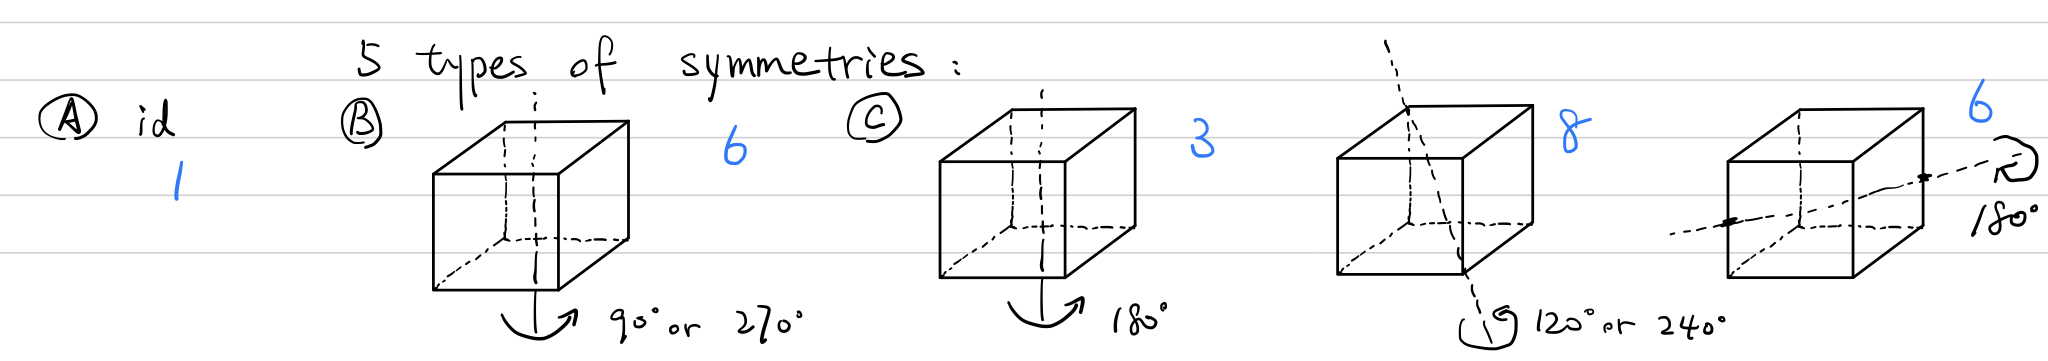
\includegraphics[width=0.7\textwidth]{Figure 2.jpg}
        \caption{\label{fig:fig2}type of rigid motions}
    \end{figure}
    Considering the action of $G$ on $A^*$, the set of uncolored labelled cubes as shown in the Figure \ref{fig:fig1}, 
    \begin{figure}[H]
        \centering
        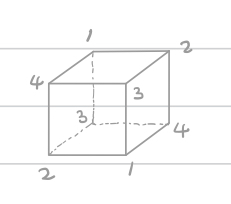
\includegraphics[width=0.3\textwidth]{Figure 1.jpg}
        \caption{\label{fig:fig1}uncolored labelled cube}
    \end{figure}
    we have the Table \ref{tab:tab2}
    \begin{table}[H]
    \centering
        \begin{tabular}{|c|c|l|l|}
        \hline
        \textbf{element of $G$} & \textbf{cycle decomposition} & \textbf{\# of cycles} & \textbf{\# of elements of this type} \\ \hline
        A                       & (1)(2)(3)(4)                 & 4                     & 1                                    \\ \hline
        B                       & (1234)                       & 1                     & 6                                    \\ \hline
        C                       & (13)(24)                     & 2                     & 3                                    \\ \hline
        D                       & (1)(234)                     & 2                     & 8                                    \\ \hline
        E                       & (1)(24)(3)                   & 3                     & 6                                    \\ \hline
        \end{tabular}
    \caption{Cycle types of $S_4$ corresponding to the rigid motion of a cube}
    \label{tab:tab2}
    \end{table}
    If we use $f(g)$ to represent the number of fixed points of $g$ acting on $A$, we know that $f(g) = k^{\text{\# cycles of g}}$. Then, by the Burnside's Lemma, we know that \# orbits $= \tfrac{1}{24}(k^4 + 6k^3 + 11k^2 + 6k) = \tfrac{k^4 + 6k^3 + 11k^2 + 6k}{24}$, i.e. there are $\tfrac{k^4 + 6k^3 + 11k^2 + 6k}{24}$ distinct ways to color the vertices of a cube using $k$ colors.
\end{answer}

\subsection{Part b}

\begin{question}
    How many distinct ways are there to color the faces of a tetrahedron using $k$ colors?
\end{question}

\begin{answer}
    First, we claim the group of rigid motions of a tetrahedron is $A_4$ if we label the tetrahedron as shown in the Figure \ref{fig:fig3}
    \begin{figure}[H]
        \centering
        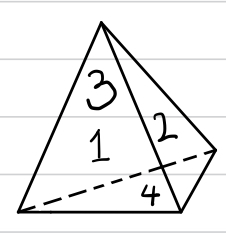
\includegraphics[width=0.2\textwidth]{Figure 3.jpg}
        \caption{\label{fig:fig3}type of rigid motions}
    \end{figure}
    To show this, we could look at the action of $A_4$ on the faces of the tetrahedron, we have the three actions described in the Figure \ref{fig:fig4}.
    \begin{figure}[H]
        \centering
        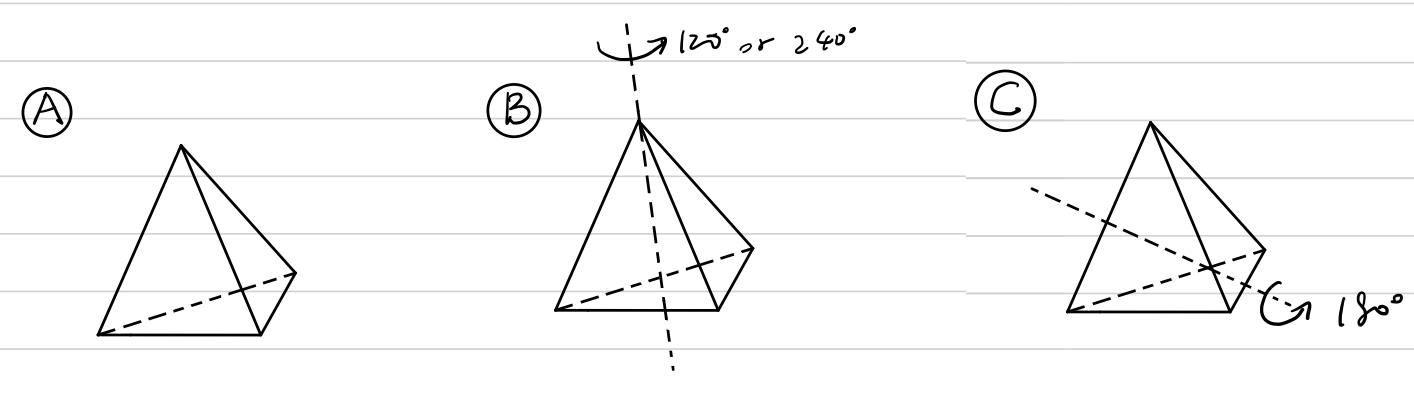
\includegraphics[width=0.7\textwidth]{Figure 4.jpg}
        \caption{\label{fig:fig4}uncolored labelled tetrahedron}
    \end{figure}
    Because we can always move a face to a face adjacent to it using action B move it to an opposite face using action C, we know that there is only one orbit, which is the set of all faces. Therefore this action is transitive. Moreover, the kernel of this actions is only the action A so that this action is faithful. Hence, we know that $Aut(\text{faces of tetrahedron}) = A_4$.
    
    Next, let $G = S_4$ acting on $A=\{$ $k$-colored labelled tetrahedron$\}$, we want to find the number of orbits of this action.
    
    Considering the action of $G$ on $A^*$, the set of uncolored labelled tetrahedron as shown in the Figure \ref{fig:fig3}, 
    
    we have the Table \ref{tab:tab3}
    \begin{table}[H]
    \centering
        \begin{tabular}{|c|c|l|l|}
        \hline
        \textbf{element of $G$} & \textbf{cycle decomposition} & \textbf{\# of cycles} & \textbf{\# of elements of this type} \\ \hline
        A                       & (1)(2)(3)(4)                 & 4                     & 1                                    \\ \hline
        B                       & (123)(4)=(13)(12)            & 2                     & 8                                    \\ \hline
        C                       & (13)(24)                     & 2                     & 3                                    \\ \hline
        \end{tabular}
    \caption{Cycle types of $S_4$ corresponding to the rigid motions of a tetrahedron}
    \label{tab:tab3}
    \end{table}
    Similar as the Part a, by the Burnside's Lemma, we know that \# orbits $= \tfrac{1}{22}(k^4 + 11k^2) = \tfrac{k^4 + 11k^2}{12}$, i.e. there are $\tfrac{k^4 + 11k^2}{12}$ distinct ways to color the vertices of a cube using $k$ colors.
\end{answer}